% 纵向模型模板
% 交叉滞后模型、潜增长模型等

\documentclass{standalone}
\usepackage{tikz}
\usetikzlibrary{shapes, arrows.meta, positioning}

% TikZ样式定义
\tikzstyle{latent} = [ellipse, draw, minimum width=2cm, minimum height=1cm]
\tikzstyle{manifest} = [rectangle, draw, minimum width=1.5cm, minimum height=0.8cm]
\tikzstyle{error} = [circle, draw, minimum size=0.6cm]
\tikzstyle{reg} = [->, >=stealth]
\tikzstyle{cov} = [<->, >=stealth]

\begin{document}

% ============================================================================
% 交叉滞后模型(CLPM)- 2波次
% ============================================================================

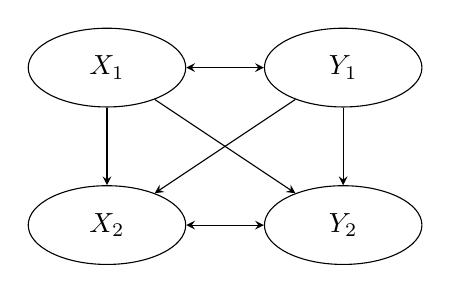
\begin{tikzpicture}
  % T1
  \node[latent] (X1) at (0,2) {$X_1$};
  \node[latent] (Y1) at (3,2) {$Y_1$};
  
  % T2
  \node[latent] (X2) at (0,0) {$X_2$};
  \node[latent] (Y2) at (3,0) {$Y_2$};
  
  % 自回归
  \draw[reg] (X1) -- (X2);
  \draw[reg] (Y1) -- (Y2);
  
  % 交叉滞后
  \draw[reg] (X1) -- (Y2);
  \draw[reg] (Y1) -- (X2);
  
  % 同期相关
  \draw[cov] (X1) -- (Y1);
  \draw[cov] (X2) -- (Y2);
\end{tikzpicture}

% ============================================================================
% 交叉滞后模型(CLPM)- 3波次
% ============================================================================

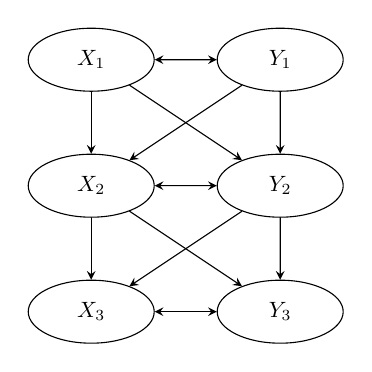
\begin{tikzpicture}[scale=0.8, transform shape]
  % T1
  \node[latent] (X1) at (0,4) {$X_1$};
  \node[latent] (Y1) at (3,4) {$Y_1$};
  
  % T2
  \node[latent] (X2) at (0,2) {$X_2$};
  \node[latent] (Y2) at (3,2) {$Y_2$};
  
  % T3
  \node[latent] (X3) at (0,0) {$X_3$};
  \node[latent] (Y3) at (3,0) {$Y_3$};
  
  % 自回归
  \draw[reg] (X1) -- (X2);
  \draw[reg] (X2) -- (X3);
  \draw[reg] (Y1) -- (Y2);
  \draw[reg] (Y2) -- (Y3);
  
  % 交叉滞后
  \draw[reg] (X1) -- (Y2);
  \draw[reg] (Y1) -- (X2);
  \draw[reg] (X2) -- (Y3);
  \draw[reg] (Y2) -- (X3);
  
  % 同期相关
  \draw[cov] (X1) -- (Y1);
  \draw[cov] (X2) -- (Y2);
  \draw[cov] (X3) -- (Y3);
\end{tikzpicture}

% ============================================================================
% 潜增长模型(LGCM)- 4个时间点
% ============================================================================

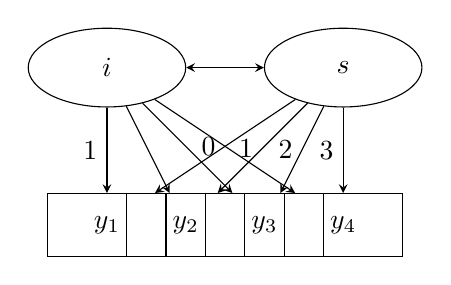
\begin{tikzpicture}
  % 潜因子
  \node[latent] (i) at (0,2) {$i$};
  \node[latent] (s) at (3,2) {$s$};
  
  % 观测变量
  \node[manifest] (y1) at (0,0) {$y_1$};
  \node[manifest] (y2) at (1,0) {$y_2$};
  \node[manifest] (y3) at (2,0) {$y_3$};
  \node[manifest] (y4) at (3,0) {$y_4$};
  
  % 截距载荷
  \draw[reg] (i) -- node[left] {$1$} (y1);
  \draw[reg] (i) -- (y2);
  \draw[reg] (i) -- (y3);
  \draw[reg] (i) -- (y4);
  
  % 斜率载荷
  \draw[reg] (s) -- node[left] {$0$} (y1);
  \draw[reg] (s) -- node[left] {$1$} (y2);
  \draw[reg] (s) -- node[left] {$2$} (y3);
  \draw[reg] (s) -- node[left] {$3$} (y4);
  
  % 协方差
  \draw[cov] (i) -- (s);
\end{tikzpicture}

% ============================================================================
% 潜增长模型(LGCM)- 二次增长
% ============================================================================

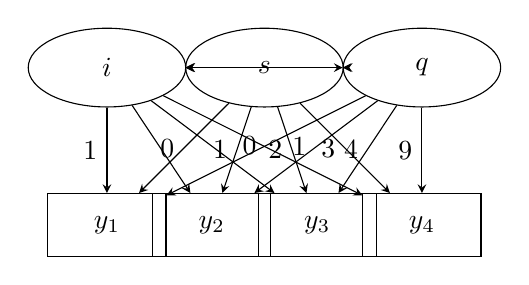
\begin{tikzpicture}
  % 潜因子
  \node[latent] (i) at (0,2) {$i$};
  \node[latent] (s) at (2,2) {$s$};
  \node[latent] (q) at (4,2) {$q$};
  
  % 观测变量
  \node[manifest] (y1) at (0,0) {$y_1$};
  \node[manifest] (y2) at (1.33,0) {$y_2$};
  \node[manifest] (y3) at (2.67,0) {$y_3$};
  \node[manifest] (y4) at (4,0) {$y_4$};
  
  % 截距载荷
  \draw[reg] (i) -- node[left] {$1$} (y1);
  \draw[reg] (i) -- (y2);
  \draw[reg] (i) -- (y3);
  \draw[reg] (i) -- (y4);
  
  % 斜率载荷
  \draw[reg] (s) -- node[left] {$0$} (y1);
  \draw[reg] (s) -- node[left] {$1$} (y2);
  \draw[reg] (s) -- node[left] {$2$} (y3);
  \draw[reg] (s) -- node[left] {$3$} (y4);
  
  % 二次项载荷
  \draw[reg] (q) -- node[left] {$0$} (y1);
  \draw[reg] (q) -- node[left] {$1$} (y2);
  \draw[reg] (q) -- node[left] {$4$} (y3);
  \draw[reg] (q) -- node[left] {$9$} (y4);
  
  % 协方差
  \draw[cov] (i) -- (s);
  \draw[cov] (i) -- (q);
  \draw[cov] (s) -- (q);
\end{tikzpicture}

% ============================================================================
% 随机截距交叉滞后模型(RI-CLPM)
% ============================================================================

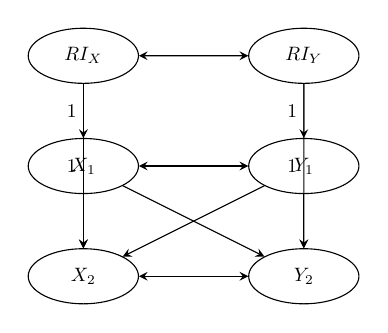
\begin{tikzpicture}[scale=0.7, transform shape]
  % 随机截距
  \node[latent] (RI_X) at (0,4) {$RI_X$};
  \node[latent] (RI_Y) at (4,4) {$RI_Y$};
  
  % T1
  \node[latent] (X1) at (0,2) {$X_1$};
  \node[latent] (Y1) at (4,2) {$Y_1$};
  
  % T2
  \node[latent] (X2) at (0,0) {$X_2$};
  \node[latent] (Y2) at (4,0) {$Y_2$};
  
  % 随机截距载荷
  \draw[reg] (RI_X) -- node[left] {$1$} (X1);
  \draw[reg] (RI_X) -- node[left] {$1$} (X2);
  \draw[reg] (RI_Y) -- node[left] {$1$} (Y1);
  \draw[reg] (RI_Y) -- node[left] {$1$} (Y2);
  
  % 自回归(状态层面)
  \draw[reg] (X1) -- (X2);
  \draw[reg] (Y1) -- (Y2);
  
  % 交叉滞后(状态层面)
  \draw[reg] (X1) -- (Y2);
  \draw[reg] (Y1) -- (X2);
  
  % 同期相关
  \draw[cov] (RI_X) -- (RI_Y);
  \draw[cov] (X1) -- (Y1);
  \draw[cov] (X2) -- (Y2);
\end{tikzpicture}

% ============================================================================
% 潜类别增长模型(LCGA)
% ============================================================================

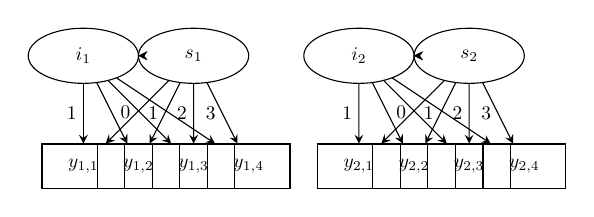
\begin{tikzpicture}[scale=0.7, transform shape]
  % 类别1
  \node[latent] (i1) at (0,2) {$i_1$};
  \node[latent] (s1) at (2,2) {$s_1$};
  \node[manifest] (y1_1) at (0,0) {$y_{1,1}$};
  \node[manifest] (y1_2) at (1,0) {$y_{1,2}$};
  \node[manifest] (y1_3) at (2,0) {$y_{1,3}$};
  \node[manifest] (y1_4) at (3,0) {$y_{1,4}$};
  
  \draw[reg] (i1) -- node[left] {$1$} (y1_1);
  \draw[reg] (i1) -- (y1_2);
  \draw[reg] (i1) -- (y1_3);
  \draw[reg] (i1) -- (y1_4);
  \draw[reg] (s1) -- node[left] {$0$} (y1_1);
  \draw[reg] (s1) -- node[left] {$1$} (y1_2);
  \draw[reg] (s1) -- node[left] {$2$} (y1_3);
  \draw[reg] (s1) -- node[left] {$3$} (y1_4);
  \draw[cov] (i1) -- (s1);
  
  % 类别2
  \node[latent] (i2) at (5,2) {$i_2$};
  \node[latent] (s2) at (7,2) {$s_2$};
  \node[manifest] (y2_1) at (5,0) {$y_{2,1}$};
  \node[manifest] (y2_2) at (6,0) {$y_{2,2}$};
  \node[manifest] (y2_3) at (7,0) {$y_{2,3}$};
  \node[manifest] (y2_4) at (8,0) {$y_{2,4}$};
  
  \draw[reg] (i2) -- node[left] {$1$} (y2_1);
  \draw[reg] (i2) -- (y2_2);
  \draw[reg] (i2) -- (y2_3);
  \draw[reg] (i2) -- (y2_4);
  \draw[reg] (s2) -- node[left] {$0$} (y2_1);
  \draw[reg] (s2) -- node[left] {$1$} (y2_2);
  \draw[reg] (s2) -- node[left] {$2$} (y2_3);
  \draw[reg] (s2) -- node[left] {$3$} (y2_4);
  \draw[cov] (i2) -- (s2);
\end{tikzpicture}

\end{document}
